\documentclass[12pt]{article}

\usepackage{graphicx,color,enumerate,multicol}
\usepackage[top=1in, bottom=1in, left=0.75in, right=1in]{geometry}
\usepackage{tikz,xcolor,pgfplots}

\usetikzlibrary{calc}
\pgfplotsset{compat=1.6}
\pgfplotsset{soldot/.style={color=black,only marks,mark=*}} \pgfplotsset{holdot/.style={color=black,fill=white,only marks,mark=*}}

%% Use Minion fonts if available.  Otherwise Times.
\IfFileExists{MinionPro.sty}{\usepackage[lf]{MinionPro}}{}
\usepackage{amsmath,amsthm,amsbsy}
\IfFileExists{MinionPro.sty}{}{\usepackage{times,txfonts}}

%% Setup aproblem environment, 
%% aproblem items
%% subproblems environment
%% subproblem items
\makeatletter
\newcounter{probcount}
\newcounter{subprobcount}
\newlength\probsep
\newlength\pshrinking
\newif\iffirstprob
\newenvironment{aproblems}%
  {\ifhmode\unskip\par\fi\setcounter{probcount}{0}\probsep\parskip
  \sbox\@tempboxa{\textbf{9.}}\pshrinking\wd\@tempboxa\advance\pshrinking\labelsep
  \let\hproblem\aproblem
  \advance\linewidth -\pshrinking
  \advance\@totalleftmargin\pshrinking
  \advance\leftskip\pshrinking}%
  {\ifhmode\unskip \par\fi\advance\leftskip-\pshrinking}%

\newcommand{\aproblem}{%
  \setcounter{subprobcount}{0}%
  \stepcounter{probcount}%
  \def\@currentlabel{\arabic{probcount}}%
  \ifhmode
    \unskip \par
  \fi
%  \addpenalty{-4000}%
  \iffirstprob\else\addvspace\probsep\fi
  \firstprobfalse
  \hskip -\labelwidth\hskip -\labelsep 
  \hbox to\labelwidth{\hss\textbf{\arabic{probcount}.}}\hskip\labelsep
}%

\newcommand{\subprob}{\item\def\@currentlabel{\arabic{probcount}\alph{\thelistlabel}}}
\newcommand{\skipproblem}{\stepcounter{probcount}}


%% The following commands put defined left and right headers on the top, and a page number
%% on the bottom of all pages beyond page 1
\usepackage{fancyhdr}
\pagestyle{fancy}
\fancyfoot[C]{\ifnum \value{page} > 1\relax\thepage\fi}
\fancyhead[L]{\ifx\@doclabel\@empty\else\@doclabel\fi}
\fancyhead[R]{\ifx\@docdate\@empty\else\@docdate\fi}
\headheight 15pt
\def\doclabel#1{\gdef\@doclabel{#1}}
\def\docdate#1{\gdef\@docdate{#1}}
\makeatother

%% General formatting parameters
\parindent 0pt
\parskip 6pt plus 1pt

\doclabel{Math F251: Section 2.2 Worksheet}
\docdate{24 January 2020}

\begin{document}
\renewcommand{\d}{\displaystyle}

\begin{aproblems}
\aproblem The function $g(x)$ is graphed below. Use the graph to fill in the blanks.

\begin{multicols}{2}
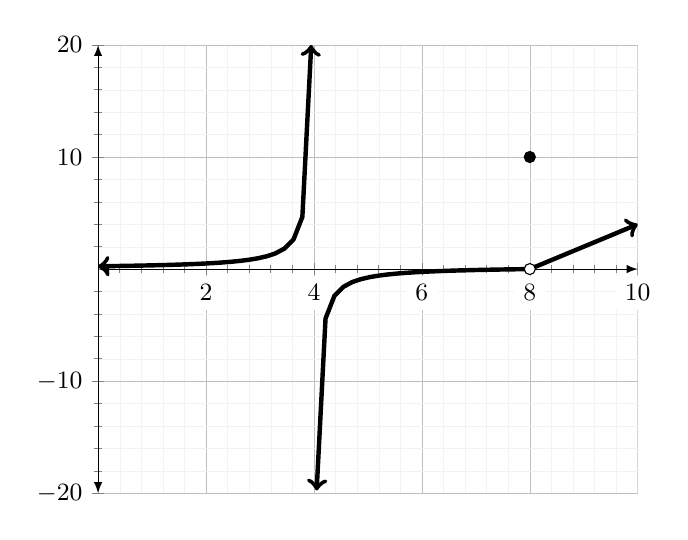
\begin{tikzpicture}[scale=1]
\begin{axis}[grid style={line width=.1pt, draw=gray!10},grid=both,major grid style={line width=.2pt,draw=gray!50},
    xmin=0,xmax=10,
    ymin=-20,ymax=20,
    xtick={},ytick={},
    minor tick num=4,
    enlargelimits={abs=0},
    ticklabel style={font=\small,fill=white},
    axis lines=middle,
    axis line style={latex-latex},
    xlabel style={at={(ticklabel* cs:1)},anchor=north west},
    ylabel style={at={(ticklabel* cs:1)},anchor=south west}
]

\addplot[<->,domain=0:3.95,ultra thick] {(4-x)^(-1)};
\addplot[<-,domain=4.05:8,ultra thick] {(4-x)^(-1)+0.25};
\addplot[->,domain=8:10,ultra thick] {2*x-16};
\addplot[soldot] coordinates{(8,10)};
\addplot[holdot] coordinates{(8,0)};
\end{axis}
\end{tikzpicture}

\columnbreak
\renewcommand{\labelenumi}{\alph{enumi})}
\begin{enumerate}
\item $\d{\lim_{x \to 4^-} g(x) = \underline{\hspace{2cm}} }$
\item $\d{\lim_{x \to 4^+} g(x) = \underline{\hspace{2cm}} }$
\item $\d{\lim_{x \to 4} g(x) = \underline{\hspace{2cm}} }$
\item $g(4)= \underline{\hspace{2cm}}$
\item $\d{\lim_{x \to 8} g(x) = \underline{\hspace{2cm}} }$
\item $g(8)= \underline{\hspace{2cm}}$
\end{enumerate}
\end{multicols}

Write the equation of any vertical asymptotes:

\vspace{20mm}

\aproblem Graph the function and then evaluate the limits:\quad $f(x)=\begin{cases} x+1 & x < 0 \\ 
x -1 & 0 \leq x < 2 \\
1+\sqrt{x-2}& 2<x \\
\end{cases}$
\vspace{2in}
\renewcommand{\labelenumi}{\alph{enumi})}
\begin{enumerate}
\item $\d{\lim_{x \to 0} f(x)}$
\vspace{.4in}

\item $\d{\lim_{x \to 2} f(x)}$
\vspace{.4in}

\item For which values $a$ does $\lim_{x \to a} f(x)$ exist?
\end{enumerate}

\newpage
\aproblem Without using a calculator, determine the (infinite) limit. Explain your reasoning.
\renewcommand{\labelenumi}{\alph{enumi})}
\begin{enumerate}
\item $\displaystyle{\lim_{x \to 3^+}\frac{\sqrt{x}}{x-3}}$\\
\vspace{.4in}

\item $\displaystyle{\lim_{x \to 3^+}\frac{{2-10x}}{\sin(x-3)}}$\\
\vspace{.4in}

\item $\displaystyle{\lim_{x \to 3^+}\ln(x-3)}$\\
\vspace{.5in}
\end{enumerate}

\aproblem Sketch the graph of a function $f$ that satisfies \emph{all} of the given conditions.  (\emph{Answers will vary.})
	\begin{enumerate}
	\item $f(0)=2$
	\item $f(3)=1$
	\item $\d{\lim_{x \to 0}f(x)}=1$
	\item $\d{\lim_{x \to 3^-} f(x)= -2}$
	\item $\d{\lim_{x \to 3^+} f(x)= 4}$
	\item $\d{\lim_{x \to -1^+}f(x)= \infty}$
	\end{enumerate}
\vfill
\end{aproblems}

\end{document}